\documentclass[10pt,twocolumn]{article}
\usepackage[letterpaper,margin=0.75in]{geometry}
\usepackage[T1]{fontenc}
\usepackage{lmodern,graphicx,booktabs,amsmath}
\usepackage[hyphens]{url}
\usepackage[hidelinks]{hyperref}
% Generated from saved result artifacts; edit the generator, not these files.

\title{Does Strict Decoding Recover Quantized Tool Calls?\\A Paired Small-Model Conceptual Replication}
\author{M. Mohith}
\date{}
\begin{document}
\maketitle
\begin{abstract}
A well-formed tool call can select the wrong function or value. We compare small Qwen and Llama models at full and quantized precision using a common GGUF engine and four decoder interventions: free generation, an unrestricted-text escape, a schema after call initiation, and whole-response enforcement. The frozen BFCL subset uses official AST and irrelevance scoring with paired item/run bootstrap intervals. On the same 60 parallel cases in a separate sensitivity, Llama-1B Q4 whole-strict parallel accuracy rises from 1.0\% to 62.3\% (paired gain 61.3 [48.7, 73.3] points); Llama-3B Q4 whole-strict parallel accuracy rises from 0.0\% to 88.3\% (paired gain 88.3 [80.0, 95.7] points). The observed format-contract gains of 61.3 and 88.3 points are much larger than the corresponding Pythonic F16-to-Q4 whole-strict gaps of 6.0 and 3.3 points. This separate sensitivity changes the prompt, parser and grammar together; it is not a randomized crossover or a parser-only causal effect. Sensitivity parallel incremental recovery and its protocol change remain inconclusive. Intervals are pointwise, unadjusted and specific to this setup. No primary free-decoding precision-loss interval excludes zero.
 We release responses, grammar checks, runtime probes, code and costs. This conceptual replication distinguishes structural guarantees from task accuracy and quantization-specific recovery.
\end{abstract}

\section{Introduction}
Local models must produce a supported representation and choose functions and arguments that answer the request. Weight compression can perturb any of these decisions. A schema removes invalid continuations but still admits incorrect actions: both Paris and London can satisfy a weather tool's city-string requirement.

TOOLDEC already enforces tool syntax without fine-tuning~\cite{tooldec}. Prior work also separates structural and content failures and studies grammar mitigation in quantized models. Our question is narrower: does strict enforcement change the \emph{incremental precision gap} differently from permissive or trigger-gated grammars? An intervention can improve a quantized model simply because it improves every precision. Conversely, a grammar with an arbitrary-text branch cannot establish a guarantee of schema-valid output. These observations motivate matched full-precision controls and an explicit check of the language each decoder admits.

We compare four interventions with paired uncertainty, retaining abstention, parallel calls and operational failures. This conceptual replication makes no priority claim about quantization damage, syntax repair or structural--semantic distinctions. The benchmark is single-turn prediction; no generated call is executed.

\section{Related work and replication scope}
Broad quantization studies emphasize dependence on the recipe and workload~\cite{bf16}. Agent diagnostics show that aggregate success can obscure process failures~\cite{flat}; decision-level analyses already investigate which tool-use decisions low-bit weights disrupt~\cite{wu}. These motivate a precision interaction, rather than a general claim that compressed models can make tool errors.

The closest software reports are QuantCall, QuantMCP and Toolhound~\cite{quantcall,quantmcp,toolhound}. Their inspected scopes differ in engine, precision controls, tasks and replication. QuantCall's default grammar unions a schema-shaped call with unrestricted text. QuantMCP describes a related escape and a forced-envelope probe with stalling. Toolhound reports trigger-gated comparisons on MLX and a custom suite. These are substantive prior experiments. Table~\ref{tab:replication} states which mechanisms we retest and what agreement would mean.

StructureBench and Chavan study structural validity and content accuracy with small models~\cite{structure,chavan}. Repair, Not Improvement isolates stopping and tool-name restrictions in a routing setting and already uses repeated runs and paired inference~\cite{repair}. JSONSchemaBench emphasizes schema coverage and efficiency~\cite{schema}. Constraint Tax highlights a separate hazard: a final-response grammar can exclude a serving protocol's tool calls~\cite{constrainttax}. We therefore constrain the declared call envelope and distinguish configuration, initiation, completion and correctness. Serving-stack differences can independently change apparent tool fidelity~\cite{serving}. Our conceptual replication retests mechanisms, without reproducing another engine or live MCP task execution.\begin{table*}[t]
\centering\footnotesize
\caption{Conceptual replication targets. Agreement concerns mechanisms under changed conditions, not prior numerical scores. Empirical directional support requires a paired interval excluding zero; otherwise that contrast remains inconclusive.}\label{tab:replication}
\begin{tabular}{p{.13\textwidth}p{.40\textwidth}p{.39\textwidth}}
\toprule
Prior work & What changes here & What would count as confirmation \\\midrule
QuantCall~\cite{quantcall} & Shared BFCL subset, prompt/compiler, paired operational schedules; add strict enforcement. & A permissive escape gives little benefit while stricter enforcement changes validity or task accuracy. A null strict effect remains a valid outcome. \\
QuantMCP~\cite{quantmcp} & Replace live MCP execution with single-turn BFCL AST scoring; preserve abstention and log completion failures. & An escape can preserve malformed output; strict generation can still fail to terminate or answer correctly. No claim to reproduce MCP task-success rates. \\
Toolhound~\cite{toolhound} & Replace MLX/custom tasks with llama.cpp/BFCL and add matched F16 controls. & Constraints improve call structure more consistently than task correctness. The added precision interaction need not match a q4-only gain. \\\bottomrule
\end{tabular}
\end{table*}


\section{Experimental design}
\subsection{Frozen tasks, models and precision}
We evaluate \texttt{Qwen3-0.6B}, \texttt{Llama-3.2-1B-Instruct}, \texttt{Llama-3.2-3B-Instruct}. The frozen sample contains 200 original cases: 60 simple, 60 multiple, 60 parallel, 20 irrelevance. The primary required-call subset contains 180 items. Each precision--decoder cell has 5 operational runs, totaling 24,000 benchmark generations in the complete matrix. Decoding uses temperature 0.0, 4 parallel server slots, a 4096-token input-plus-output budget per request, and an output cap of 512 tokens.

The same original items and accepted answers are retained across all conditions. Selection does not depend on baseline success, validity or a model prediction. The pilot subset was used for runtime and cost calibration, not to choose favorable tasks. Full-run prompts are frozen from publisher tokenizers and chat templates; the Llama template date is fixed. The common Qwen pilot prompts and whole-response grammars match the corresponding full-run inputs.

Weights are exported once to F16 GGUF and the quantized artifact is generated directly from that export. This reference is an F16 export, not the original checkpoint's possibly different storage dtype. Both K and V caches stay F16. Qwen thinking is disabled~\cite{qwencard}. Model revisions, source/output hashes, conversion commands, server arguments and the pinned llama.cpp source~\cite{llamacpp} are recorded. All arms and precisions for a model use one A10 worker. The Modal allocation selector is fixed. Device-reported A10/A10G labels and drivers are retained rather than normalized away; model sessions need not share a physical host.

\subsection{Decoder languages and prompt contract}
Every arm for a given model sees exactly the same rendered prompt and offered tools. The primary Llama prompts use the single-object JSON tool branch of \texttt{tokenizer\_config.json}'s embedded HF chat template, with \texttt{tools\_in\_user\_message=True}. Both selected revisions have the same template hash, recorded in Appendix~\ref{app:settings}. We added a JSON-array convention for parallel calls in the system message, while that HF template inserts a later user-message instruction requesting one JSON object. These instructions conflict on parallel tasks. Meta separately documents a Pythonic list of calls~\cite{metaprompt}; our primary JSON contract does not evaluate that format. Llama findings are conditional on this declared contract, rather than claims about its best supported interface. Qwen uses tagged call objects with \texttt{name} and \texttt{arguments}; Llama uses objects with \texttt{name} and \texttt{parameters}, or arrays for parallel calls. All arms use \texttt{NO\_CALL} when no offered tool applies. The grammar never uses the expected function, accepted values or gold call count.

\textbf{Free} applies no grammar. \textbf{Loose} unions the schema-shaped language with arbitrary text, reproducing the escape as a control. \textbf{Trigger-strict} leaves initiation unconstrained and activates the call language at the declared prefix. Qwen uses its preserved call token; Llama uses one pattern matching the earliest object or array opener, including an opener merged into a token. \textbf{Whole strict} admits only a documented call sequence or the explicit no-call form. Parallel-call count and order are not fixed to the reference. Lazy activation can encounter a merged trigger-containing token whose remainder violates the call language. Known replay errors are retained as failed attempts, rather than retried or admitted through a grammar escape.

The compiler permits arbitrary ordering of documented object keys while enforcing required/unique keys. Known property sets are closed as an explicit API policy. Free-form dictionaries remain free-form. A nested BFCL dictionary that names required fields without field types retains those names with unconstrained values; types are not guessed from answers. These normalization choices are part of the intervention and are released.

Finite character-level membership checks cover the selected schemas, malformed strings, unknown functions, missing/extra arguments, types, key order, parallel calls and abstention. They are evidence of tested coverage, not a proof of every JSON Schema feature or token-level behavior. Separate synthetic runtime probes force a known trigger and verify literal replay and the server's configured lazy mode before benchmark collection. These probes are setup, not benchmark successes. No engine patch is used.

\subsection{Execution and scoring}
Temperature is zero, with seed/schedule labels frozen before execution and shuffled requests. Identical greedy outputs are retained as operational repeats; they are not new independent items. Configured context/output caps, server slots, cache settings and stop strings match across arms. Grammar acceptance itself changes when termination is legal. Llama prompts use publisher token IDs to avoid duplicating the beginning-of-text marker already present in its template. An earlier collection with that duplication is retained as an aborted setup attempt, before task-accuracy inspection. Qwen uses its original string transport with publisher settings that disable added BOS. Cache-reuse timings and actual generation settings are logged. The cloud supervisor checkpoints events, enforces queue/runtime bounds and enforces the scheduling rule frozen before execution. The researcher permitted concurrent full studies after the separate pilots; this does not establish isolated cross-model throughput.

Official BFCL AST matching is the correctness authority~\cite{bfcl}. We adapt the declared JSON envelope into calls without executing outputs. The pinned checker is unmodified; a minimal registry entry supplies its name-normalization flag without importing unrelated API clients. The unchanged official irrelevance helper is used through the same parsing adapter. Irrelevance can credit an output with no parsed call while our format diagnostic rejects its prose; those outcomes are reported separately. Required-call accuracy is the primary endpoint.

Our deterministic diagnostics retain multiple flags and an ordered primary label: format failure, wrong or hallucinated function, missing/extra or hallucinated arguments, wrong type and wrong value, plus missing/extra calls and operational statuses. A schema-valid parallel mismatch is not labeled a known value error without evidence from the checker. Incomplete output and runtime failures remain visible. Unstarted budget-censored cells are reported as incomplete, rather than filled with synthetic predictions.

\subsection{Estimands and paired uncertainty}
Let $A_{p,d}$ be official item accuracy at precision $p$ and decoder $d$, with $f$ denoting free decoding. For the quantized precision $q$, define
\begin{align}
 L_f &= A_{\mathrm{F16},f}-A_{q,f},\\
 L_d &= A_{\mathrm{F16},d}-A_{q,d},\\
 R_d &= L_f-L_d.
\end{align}
$R_d$ removes the decoder effect already present at F16. We also compare $R_{\mathrm{whole}}-R_{\mathrm{loose}}$ and the corresponding trigger contrast on paired observations. These are intervention effects, not an identified fraction of purely syntactic knowledge loss: schemas restrict names, keys and types, and can redirect subsequent value choices.

Primary percentile intervals use crossed paired resampling of original item IDs and operational-run labels, sharing draws across all conditions and models. Item-only intervals are saved as a sensitivity check. Category rates use their original item subsets. Intervals are pointwise and unadjusted for multiple comparisons; exploratory contrasts are labeled accordingly. At a boundary with no observed failures, empirical bootstrap intervals can degenerate; this is not a bound on rare unobserved population failures. A recovery-share point estimate $R_d/L_f$ is undefined when observed free loss is nonpositive. Its interval is withheld when bootstrap denominators are unstable; values are not clipped into a manufactured partition.

\section{Results}
Qwen3-0.6B: Q4 required-call accuracy changes from 70.7\% free to 75.6\% whole strict. Its incremental recovery is 2.1 [-0.7, 5.2] percentage points. Across all cases for Qwen3-0.6B, Q4 whole-strict response-structure validity is 100.0 [100.0, 100.0]\%, while official accuracy is 73.0 [66.9, 79.0]\%.

Llama-3.2-1B: Q4 required-call accuracy changes from 14.2\% free to 52.7\% whole strict. Its incremental recovery is -4.7 [-9.1, -0.3] percentage points. Across all cases for Llama-3.2-1B, Q4 whole-strict response-structure validity is 100.0 [100.0, 100.0]\%, while official accuracy is 47.4 [40.5, 54.2]\%. Its Q4 whole-strict parallel accuracy under the declared JSON contract is 1.0 [0.0, 4.0]\%. This does not measure the publisher Pythonic call-list contract.

Llama-3.2-3B: Q4 required-call accuracy changes from 29.2\% free to 61.0\% whole strict. Its incremental recovery is -2.1 [-5.0, 0.6] percentage points. Across all cases for Llama-3.2-3B, Q4 whole-strict response-structure validity is 100.0 [100.0, 100.0]\%, while official accuracy is 54.9 [48.0, 61.7]\%. Its Q4 whole-strict parallel accuracy under the declared JSON contract is 0.0 [0.0, 0.0]\%. This does not measure the publisher Pythonic call-list contract.

Generation status counts are grammar\_trigger\_replay\_error: 1; ok: 23860; token\_limit: 139. Negative incremental recovery does not mean constraints lowered Q4 accuracy: they helped F16 more in these cells. Valid structure includes no-call responses; task correctness and irrelevance are scored separately. Other diagnostic rates, category endpoints, item-only sensitivity intervals, paired decoder contrasts and raw responses are released with the result tables. Intervals crossing zero do not establish equivalence.

\begin{table*}[t]
\centering\scriptsize
\caption{Required-call accuracy (\%) and crossed paired 95\% intervals. Repeated schedules remain clustered with original items.}
\begin{tabular}{llrrrr}
\toprule
Model & Precision & Free & Loose & Triggered & Whole strict \\
\midrule
Qwen3-0.6B & F16 & 73.9 [67.2, 80.0] & 73.9 [67.2, 80.0] & 76.7 [70.0, 82.8] & 76.7 [70.0, 82.8] \\
Qwen3-0.6B & Q4\_K\_M & 70.7 [64.0, 77.0] & 70.7 [63.9, 77.0] & 74.8 [68.4, 80.7] & 75.6 [69.2, 81.4] \\
Llama-3.2-1B & F16 & 12.8 [8.3, 17.8] & 12.8 [8.3, 17.8] & 54.3 [47.1, 61.7] & 55.9 [48.7, 63.1] \\
Llama-3.2-1B & Q4\_K\_M & 14.2 [9.3, 19.4] & 14.1 [9.2, 19.4] & 51.9 [44.7, 59.1] & 52.7 [45.3, 59.9] \\
Llama-3.2-3B & F16 & 27.2 [20.6, 33.9] & 27.2 [20.6, 33.9] & 61.1 [53.9, 68.3] & 61.1 [53.9, 68.3] \\
Llama-3.2-3B & Q4\_K\_M & 29.2 [22.7, 35.9] & 29.4 [22.8, 36.1] & 60.4 [53.3, 67.6] & 61.0 [53.9, 68.1] \\
\bottomrule
\end{tabular}

\end{table*}
\begin{figure*}[t]
\centering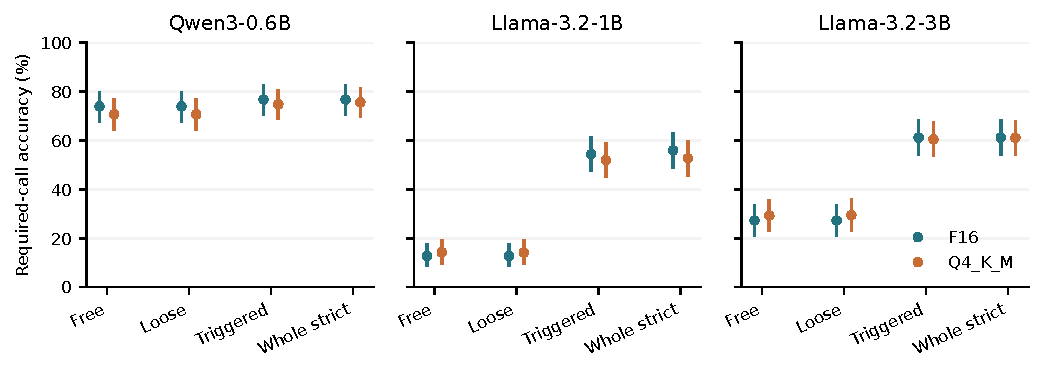
\includegraphics[width=\textwidth]{../figures/accuracy.pdf}
\caption{Required-call accuracy under each intervention. Whiskers are crossed paired bootstrap intervals, not independent-binomial intervals over repeated generations.}
\end{figure*}
\begin{figure*}[t]
\centering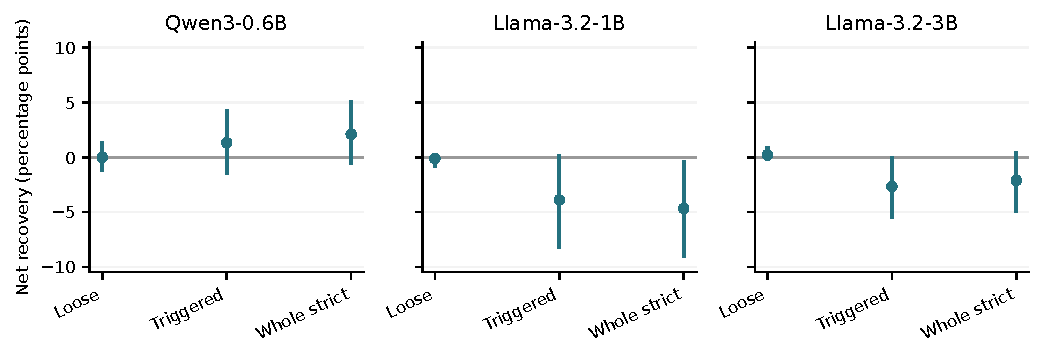
\includegraphics[width=\textwidth]{../figures/net_recovery.pdf}
\caption{Signed recovery of the incremental F16--Q4 gap. Zero means no observed reduction of that gap; negative effects are retained. This quantity does not causally separate syntax from semantics.}
\end{figure*}
\begin{table*}[t]\centering\scriptsize
\caption{Required-call signed precision loss and incremental recovery, in percentage points [95\% CI]. The final column is the normalized share (\%) when its denominator is stable.}
\begin{tabular}{llrrrr}\toprule
Model & Decoder & Free loss & Constrained loss & Net recovery & Recovery share \\\midrule
Qwen3-0.6B & Loose & 3.2 [-1.9, 8.3] & 3.2 [-1.9, 8.3] & 0.0 [-1.3, 1.4] & unstable \\
Qwen3-0.6B & Triggered & 3.2 [-1.9, 8.3] & 1.9 [-2.4, 6.2] & 1.3 [-1.6, 4.3] & unstable \\
Qwen3-0.6B & Whole strict & 3.2 [-1.9, 8.3] & 1.1 [-3.2, 5.3] & 2.1 [-0.7, 5.2] & unstable \\
Llama-3.2-1B & Loose & -1.4 [-4.4, 1.4] & -1.3 [-4.4, 1.6] & -0.1 [-0.9, 0.3] & undefined \\
Llama-3.2-1B & Triggered & -1.4 [-4.4, 1.4] & 2.4 [-1.8, 6.7] & -3.9 [-8.3, 0.2] & undefined \\
Llama-3.2-1B & Whole strict & -1.4 [-4.4, 1.4] & 3.2 [-0.7, 7.2] & -4.7 [-9.1, -0.3] & undefined \\
Llama-3.2-3B & Loose & -2.0 [-4.6, 0.3] & -2.2 [-4.9, 0.2] & 0.2 [-0.3, 1.0] & undefined \\
Llama-3.2-3B & Triggered & -2.0 [-4.6, 0.3] & 0.7 [-0.8, 2.2] & -2.7 [-5.6, 0.1] & undefined \\
Llama-3.2-3B & Whole strict & -2.0 [-4.6, 0.3] & 0.1 [-1.3, 1.4] & -2.1 [-5.0, 0.6] & undefined \\
\bottomrule\end{tabular}\end{table*}

\paragraph{Separate Pythonic-format sensitivity.} We additionally collected 4,800 responses on 120 frozen cases, using the original parallel subset plus a separately sampled parallel-multiple subset, both Llama models, both precisions, free/whole strict and the same operational labels. The prompt follows Meta call-list syntax, omits the HF tools injection, and uses [] for abstention. Llama-3.2-1B Q4 whole-strict parallel accuracy is 62.3 [50.0, 74.3]\%, versus 1.0\% under the original JSON contract. Its Pythonic parallel incremental recovery is 1.7 [-10.3, 13.7] points; the paired change in recovery versus JSON is 2.3 [-10.0, 15.0] points; Llama-3.2-3B Q4 whole-strict parallel accuracy is 88.3 [80.0, 95.7]\%, versus 0.0\% under the original JSON contract. Its Pythonic parallel incremental recovery is -3.3 [-8.7, 0.7] points; the paired change in recovery versus JSON is -3.3 [-8.7, 0.7] points. These gains change the interpretation of the low primary Llama parallel scores: they are strongly contract-dependent, rather than evidence of an intrinsic inability to make parallel calls. Neither parallel incremental recovery nor its protocol change is resolved from zero. This is a joint prompt/parser/grammar sensitivity, not a parser-only causal estimate. Only the original parallel items have a matched primary baseline; parallel-multiple results are reported separately. Sessions differ in time and host, so this is not a randomized crossover. Llama-3B was interrupted by the platform after 1,610 durable outputs; only the missing 790 cells continued on another A10, with saved failures retained. The primary matrix is unchanged. Additional status counts are ok: 4222; token\_limit: 578. These limits remain incorrect; no added exclusion analysis is claimed.


\section{Cost, limitations and practical implications}
The pilot-based cost forecast for the primary campaign was \$4.74--\$8.14. Before the follow-up, reported gross project spending was \$2.6110, including setup and interrupted attempts, against the \$12.00 cap. These are reported charges, not a settled invoice. Final app and container shutdown records are stored separately from the billing snapshot.
The separate Pythonic sensitivity added \$0.7346, including failed and interrupted apps, bringing reported project spending to \$3.3456, within the additional \$3.00 and total \$12.00 caps.

Forecasts are assumptions rather than observations. Timed estimates omit untimed platform stages; metering can lag and does not establish storage completeness. Earlier failures remain in the release.

This small frozen BFCL sample is not a complete leaderboard evaluation. AST correctness does not establish safe execution, successful multi-turn agents, or correctness on unseen APIs. Irrelevance has a small diagnostic sample. The inference stack, cache dtype, weight recipe, output envelope and schema normalization are fixed; results do not automatically extend to other quantizers, KV-cache compression, larger catalogs or different engines. Prefix triggering is an operational rule, not a direct measure of internal intent. Log-derived activation is distinguished from a direct trace of sampler state.

\paragraph{Primary failures and post-hoc exclusion.} Qwen3-0.6B has 0 token-limit outcomes and 0 replay errors; Llama-3.2-1B has 101 token-limit outcomes and 1 replay error; Llama-3.2-3B has 38 token-limit outcomes and 0 replay errors. Failures cluster by decoder and task; exclusion may depend on treatment or difficulty. The analysis frozen before execution counts failures as incorrect. Three sensitivity checks exclude failures per cell, remove a model--item--run from all precision--decoder cells if any cell failed, or remove whole items with any failure. The second rule preserves a common observed cohort; its required-call whole-strict recovery is Qwen3-0.6B 2.1 [-0.7, 5.2]; Llama-3.2-1B -4.8 [-9.4, -0.5]; Llama-3.2-3B -2.1 [-5.1, 0.6] percentage points [95\% CI]. Across all three rules and both endpoints, directional interval classifications change for 0 recovery effects and 0 decoder contrasts. Cell-only exclusion changes the completed population; all three select on a post-treatment outcome and may favor easier items. None estimates performance with unlimited generation or a repaired engine. The failure report gives every cell count, retained denominator and supplementary interval; primary results remain unchanged.


Closed schemas can forbid useful undocumented arguments; typed allowed values can still be wrong. Parser policy affects prose, abstention and parallel-call scoring. Operational repeats do not resample training runs, quantization builds or templates, or establish generalization across hardware. Intervals crossing zero do not prove equality.

Operators need task accuracy under the same serving contract and a matched high-precision control. Structural guarantees remain useful without accuracy gains. The planned Direction 2 follow-up compares schema-audit/precision fallback with ordinary retries; it is not evaluated here.

\section{Conclusion}
The separate sensitivity shows that the tool-call format contract has a much larger observed accuracy contrast than weight precision in this setup. Llama-1B Q4 whole-strict parallel accuracy rises from 1.0\% to 62.3\%; Llama-3B Q4 whole-strict parallel accuracy rises from 0.0\% to 88.3\%. This changes the interpretation of the low primary Llama parallel scores, while leaving the primary matrix unchanged. The comparison changes prompt, parser and grammar together. Sensitivity parallel incremental recovery and its protocol change remain inconclusive. The pointwise, unadjusted intervals do not establish recovered quantization damage. No primary free-decoding precision-loss interval excludes zero.

\appendix
\section{Settings and availability}\label{app:settings}
Code, frozen data, responses, analysis and the paper are at \url{https://github.com/mohi-devhub/grammar-vs-bits}. The primary campaign is \texttt{full-002}; the Pythonic sensitivity is separate. The design was frozen before execution, without a public preregistration timestamp. The code is MIT licensed; redistributed BFCL material includes Gorilla's Apache-2.0 license and attribution.

BFCL v4 data and checker are pinned to Gorilla revision \texttt{6ea57973c7a6097f}\allowbreak\texttt{d7c5915698c54c17}\allowbreak\texttt{c5b1b6c8}. The engine is llama.cpp revision \texttt{8542e94350f0ade0}\allowbreak\texttt{1644db6f1d1520da}\allowbreak\texttt{3814dafd}. Crossed bootstrap intervals use 10,000 draws and seed 20261028. Operational labels are 101, 211, 307, 401 and 503. Qwen uses \texttt{enable\_thinking=False}. Each model loads F16 first and Q4 second, with the five shuffled schedules inside each precision block; precision order was not counterbalanced. These intervals describe item/schedule variation under that execution.

The Llama HF JSON templates are from 1B revision \texttt{9213176726f574b5}\allowbreak\texttt{56790deb65791e0c}\allowbreak\texttt{5aa438b6} and 3B revision \texttt{0cb88a4f764b7a12}\allowbreak\texttt{671c53f0838cd831}\allowbreak\texttt{a0843b95}. Their template SHA-256 is \texttt{2732d9da5568668e}\allowbreak\texttt{d22ea202bffb12f0}\allowbreak\texttt{df405439651e1275}\allowbreak\texttt{ba1f521522f92966}. Exact executed worker sources and hash records are in \texttt{provenance/}; the maintained implementation is separate. Historical launcher revisions were not retained, so we do not claim to have recovered them. Prompts and per-run commands are released.

\bibliographystyle{plain}
{\small\bibliography{references}}
\end{document}
